\chapter{Revisión de técnicas}

En este capítulo se describen los procesos y algoritmos utilizados a lo largo del trabajo descrito en esta memoria. Concretamente, se comienza explicando el concepto de la \textbf{ciencia de datos} y su ciclo de vida, haciendo énfasis en \textbf{CRISP-DM} como metodología utilizada a lo largo del proyecto para resolver el problema propuesto. Tras esto, se estudian conceptos de aprendizaje automático como los \textbf{modelos de regresión} - haciendo especial énfasis en los modelos de \textit{ensemble} basados en técnicas de \textbf{\textit{Gradient Boosting}} - o la búsqueda de hiperparámetros.


\section{Ciencia de datos y el ciclo de vida de los datos}

La \textbf{ciencia de datos} es el estudio de la extracción de conocimiento útil a partir de datos, y de la generalización de dicho proceso a cualquier problema \cite{Donoho02102017}. Dicho proceso incluye la recolección y almacenamiento, mantenimiento, procesamiento, análisis y visualización de enormes cantidades de datos heterogéneos - asociados a un gran abanico de aplicaciones y dominios en muchas ocasiones multidisciplinarios \cite{10.1145/2500499}.

Desde su origen, la ciencia de datos ha evolucionado como un campo interdisciplinar que integra conocimientos y técnicas de otras disciplinas afines como el análisis de datos, la estadística o la minería de datos \cite{potential}. Ahora bien, la principal diferencia con estos campos se encuentra en el fin: el aprendizaje a partir de los datos \cite{Donoho02102017} y la capacidad de adquirir nuevo conocimiento capaz de ser utilizado para la toma de decisiones y la predicción \cite{10.1145/2500499}.

\begin{figure}[h]
	\centering
	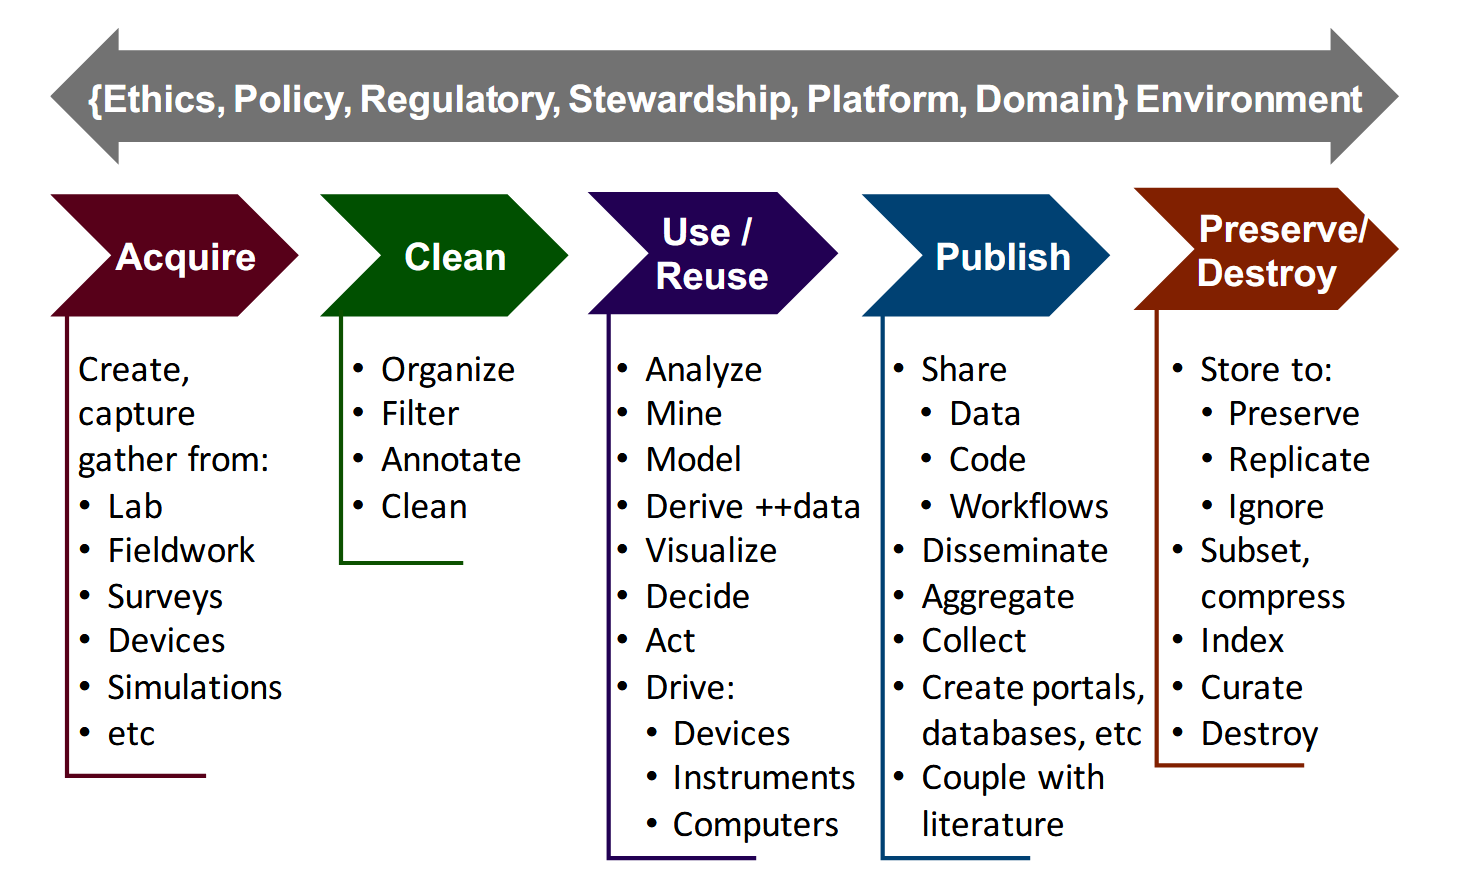
\includegraphics[width=0.8\linewidth]{figs/chapter2/datalifecycle}
	\caption{Ciclo de vida de los datos \cite{potential}}
	\label{fig:datalifecycle}
\end{figure}

Por definición, la ciencia de datos depende de los datos sobre los que se está trabajando. Por esto, el proceso de trabajo de la ciencia de datos depende generalmente del \textbf{ciclo de vida de los datos}: las distintas etapas por las que pasa un conjunto de datos desde su recolección e investigación hasta su uso final \cite{datasciencelifecycle}. Como se observa en la \textbf{Figura \ref{fig:datalifecycle}}, este ciclo está tradicionalmente dividido en \textbf{cinco} apartados \cite{potential}:



\begin{enumerate}
	\item \textbf{Adquisición:} En la actualidad, los datos se generan en cantidades masivas - del orden de \textbf{exabytes por hora} \cite{Wing2019Data}. Por tanto, el primer paso del ciclo consiste en la adquisición y almacenamiento eficiente de los datos necesarios para el proceso.
	\item \textbf{Limpieza:} Tras la adquisición, el segundo paso del ciclo consiste en la transformación de los datos originales en datos utilizables posteriormente - a través de procesos de limpieza, imputación, formateo...
	\item \textbf{Uso y re-uso:}  El tercer paso del ciclo consiste en el uso de los datos procesados con el fin de adquirir conocimiento y tomar decisiones a partir de éstos. Éste apartado se puede dividir, a su vez, en tres subapartados \cite{Wing2019Data}:
		\begin{enumerate}
			\item \textbf{Análisis exploratorio:} El estudio del comportamiento de los datos con el fin de plantear hipótesis para guiar el resto del ciclo de datos \cite{eda}.
			\item \textbf{Modelado:} El uso de técnicas computacionales y estadísticas para extraer conocimiento y predicciones a partir del conjunto de datos.
			\item \textbf{Visualización, interpretación y actuación:}  La representación gráfica de los resultados del uso de los datos, con el fin de facilitar la toma de decisiones posterior a las personas.
		\end{enumerate}
	\item \textbf{Publicación:} El cuarto paso del ciclo consiste en la diseminación de los resultados del proceso - con el fin de que el conocimiento creado pueda ser conocido y reutilizado por el mayor número de personas posible.
	\item \textbf{Preservación o destrucción:} El quinto y último paso del ciclo consiste en la preservación o destrucción de los datos utilizados - cumpliendo con otros factores como pueden ser las consideraciones éticas o regulatorias.
\end{enumerate}

Con el fin de regularizar, estandarizar y hacer reproducible el proceso completo de la ciencia de datos - desde la adquisición de los conjuntos de datos hasta la distribución de los resultados -, se han propuesto varias ampliaciones y adaptaciones del ciclo de datos estudiado, conocidas como \textbf{ciclos de vida de la ciencia de datos} \cite{datasciencelifecycle}. 

Aunque actualmente no existe un ciclo estandarizado, uno de los procesos más utilizados para ciencia de datos es el \textbf{Cross-Industry Standard Process for Data Mining (\textit{CRISP-DM})}, propuesto originalmente para el campo de la minería de datos pero adaptado a las necesidades de la ciencia de datos \cite{shearer2000crisp}.

\subsection{Cross-Industry Standard Process for Data Mining - CRISP-DM}

\textbf{Cross-Industry Standard Process for Data Mining} (abreviado como \textit{CRISP-DM}) es una metodología desarrollada con el fin de ofrecer un proceso de trabajo completo de principio a fin para la minería de datos; independientemente del campo, las herramientas o la aplicación final de los datos \cite{shearer2000crisp}. Si bien fue propuesto originalmente en el año 2000, en la actualidad sigue siendo uno de los procesos más utilizados tanto en minería de datos como en ciencia de datos \cite{Mariscal_Marbán_Fernández_2010} \cite{datasciencepmCRISPDMStill}.

\begin{figure}[h]
	\centering
	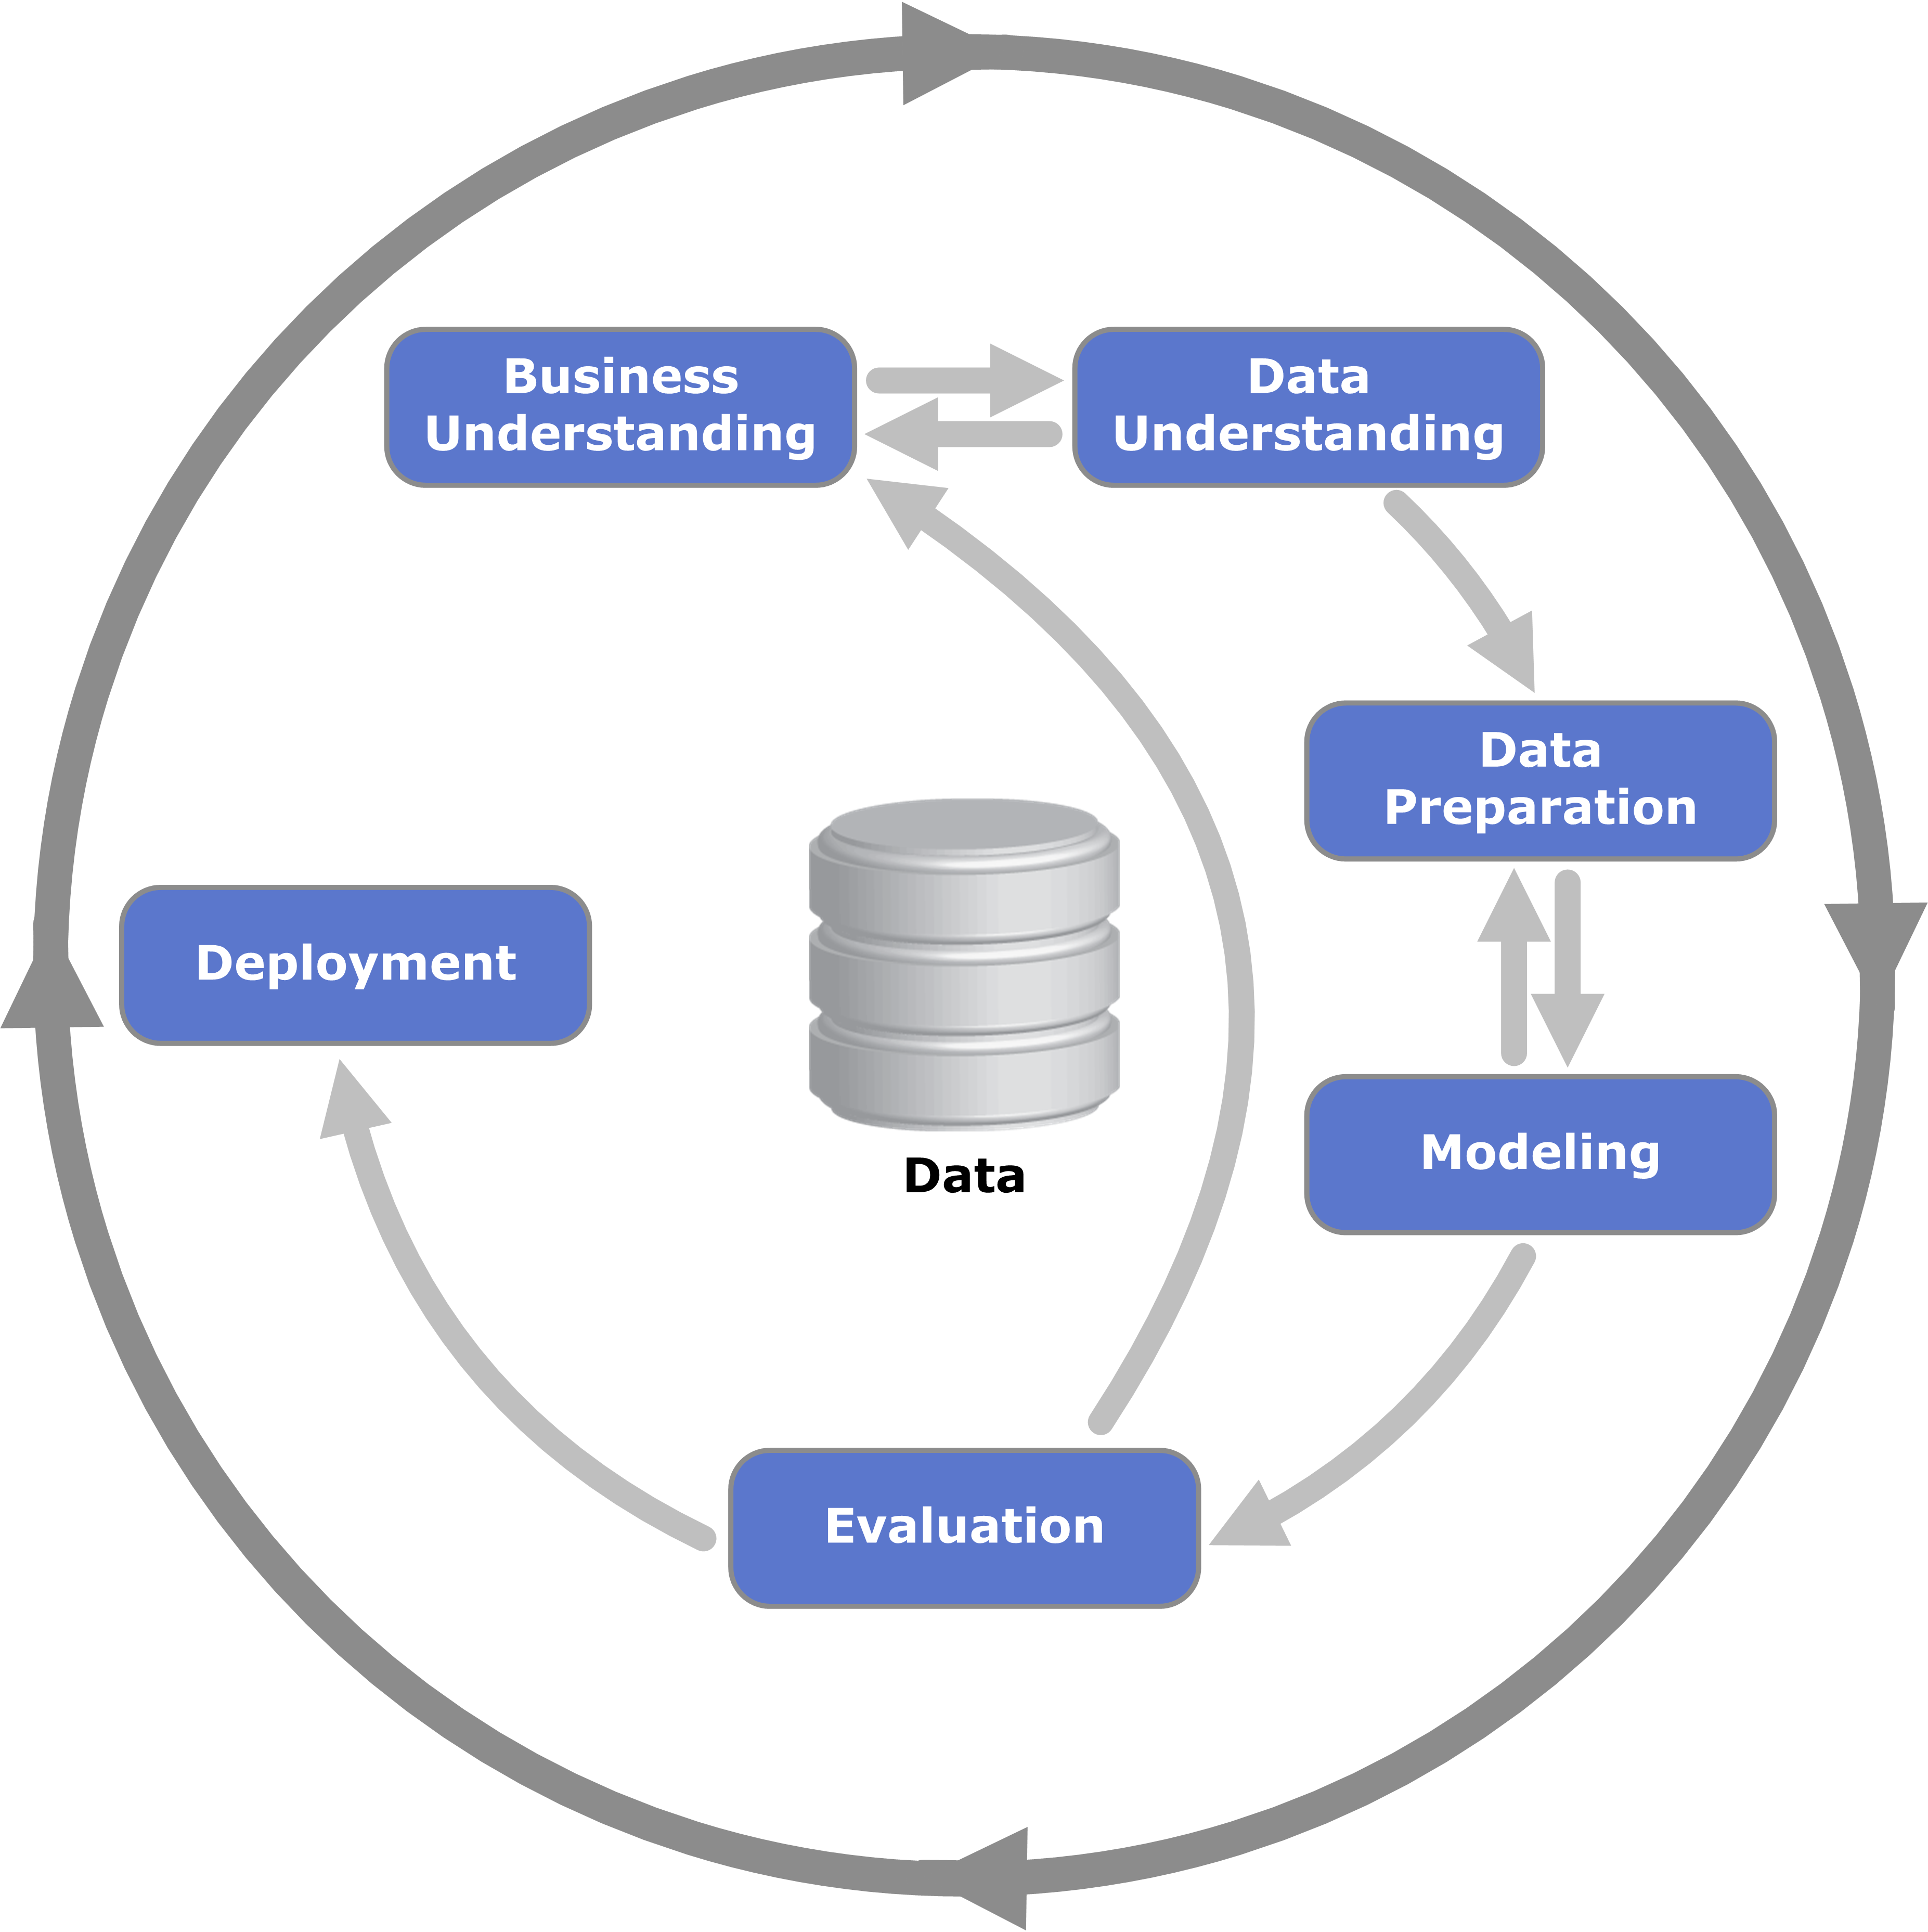
\includegraphics[width=0.6\linewidth]{figs/chapter2/crispdm}
	\caption{Ciclo de vida de CRISP-DM \cite{shearer2000crisp}}
	\label{fig:crispdm}
\end{figure}

Como se observa en la \textbf{Figura \ref{fig:crispdm}}, el ciclo de CRISP-DM está dividido en \textbf{seis fases} \cite{shearer2000crisp}, similares al ciclo de datos estudiado:

\begin{enumerate}
	\item \textbf{Conocimiento del campo (\textit{Business Understanding}):} El primer paso del ciclo consiste en entender el problema y los objetivos a resolver - estudiando la situación actual y estableciendo los pasos para alcanzar las metas propuestas.
	\item \textbf{Conocimiento de los datos (\textit{Data Understanding}):} El segundo paso del ciclo consiste en adquirir y estudiar los datos - tanto de forma superficial como en un análisis exploratorio más profundo -, además de verificar que los datos disponibles son útiles para los objetivos propuestos.
	\item \textbf{Preparación de los datos (\textit{Data Preparation}):} Tras la adquisición de conocimiento, el tercer paso consiste en preparar los datos obtenidos para su uso posterior - seleccionando las instancias relevantes, limpiando los datos para eliminar valores perdidos, enriqueciendo los datos con información externa...
	\item \textbf{Modelado (\textit{Modeling}):} Con los datos preparados, la cuarta fase del ciclo consiste en el uso y calibración de modelos de aprendizaje automático - definiendo los estudios y experimentos a realizar sobre los modelos, y evaluando el rendimiento final de éstos.
	\item \textbf{Evaluación (\textit{Evaluation}):} Antes de desplegar el modelo final, la quinta fase del ciclo consiste en evaluar si los resultados obtenidos satisfacen los objetivos propuestos y si el proceso de ciencia de datos se ha aplicado de forma adecuada.
	\item \textbf{Despliegue (\textit{Deployment}):} La última fase del ciclo es el despliegue y diseminación de los resultados obtenidos - haciendo disponible el modelo y los resultados a los usuarios finales.
	
\end{enumerate}

Es importante destacar que, como indican las flechas de la \textbf{Figura \ref{fig:crispdm}}, la metodología propuesta no es linear, sino que el flujo entre los distintos pasos se puede ver alterado:
\begin{itemize}
	\item Las fases tienen dependencias entre sí - los descubrimientos en algunas fases pueden producir que sea necesario volver a fases anteriores para perfeccionar el proceso.
	\item El proceso es \textbf{cíclico} - los conocimientos adquiridos durante las distintas fases se aplican para refinar futuros procesos, ya sean sobre el mismo conjunto de datos o datos nuevos.
\end{itemize}


\section{Aprendizaje supervisado y modelos de regresión}

\subsection{Modelos simples}

\subsubsection{Modelos de regresión lineal}

\subsubsection{Árboles de decisión}

\subsubsection{Máquinas de vectores de soporte}

\subsection{Modelos grupales - Ensembles}

\subsubsection{Bagging}

\subsubsection{Boosting}

\subsubsection{Gradient Boosting}

\subsection{Ajuste de hiperparámetros y validación cruzada}
